%auteur: Amaury JOLY
\begin{frame} 
  \frametitle{Qu’est-ce qu’une sidechain ?} 
  \begin{itemize} 
    \item Une blockchain secondaire 
    \item Parallèle à une blockchain principale 
    \item Propres caractéristiques 
    \item Sécurité et communauté du réseau principal 
  \end{itemize} 

  \begin{figure}
    \centering
    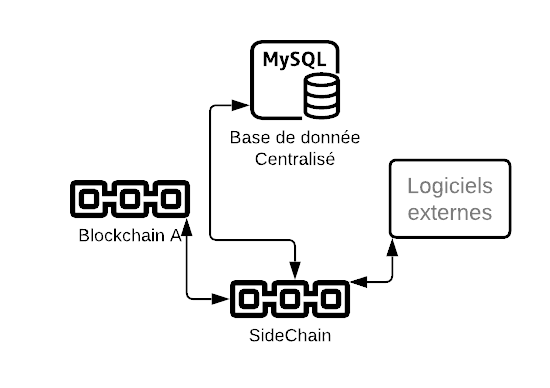
\includegraphics[scale = 0.4]{decentralisation/sidechain.png}
    \caption{Sidechain}
  \end{figure}
\end{frame}

\begin{frame} 
  \frametitle{Qu’est-ce que Zendoo ?} 
  \begin{itemize} 
    \item Il permet la création de sidechains interopérables avec la blockchain Horizen 
    \item Il propose un protocole de transfert cross-chain sans divulgation d'informations. 
    \item Atouts:
    \begin{itemize}
      \item Systèmes sans commission à l'usage.
      \item Peut s'interfacer à d'autres systèmes que la Blockchain.
    \end{itemize}
  \end{itemize} 
\end{frame}

\begin{frame} 
  \frametitle{Quelle sont les contraintes techniques des sidechains ?} 
  \begin{itemize} 
    \item Avantages:
    \begin{itemize}
      \item Présente une intéropérabilité maximale.
    \end{itemize}
    \item Inconvénients:
    \begin{itemize}
      \item Contraintes techniques pour la mise en place avec des blockchains existantes.
      \begin{itemize}
        \item Enjeu sur la création d’un pont bidirectionnel.
        \item Le compatibilité des actifs entre les deux chaînes n'est pas évidente. 
        \item La coordination entre deux chaînes techniquement trés éloignées est impossible.
      \end{itemize}
      \item Problèmes de sécurité, de performance ou de compatibilité délégué à une seule chaine.
    \end{itemize}
  \end{itemize} 
\end{frame}